\documentclass[10pt,spanish,a4paper,openany,notitlepage]{article}
%-------------------------------------Paquetes-----------------------------------------------------------------------
\usepackage[spanish,es-tabla]{babel}  	% Traduce los textos a castellano
\usepackage[utf8]{inputenc}	% Permite escribir directamente áéíóúñ
\usepackage{t1enc}            	% Agrega caracteres extendidos al font
\usepackage{amsmath} 		%Permite imprimir mas opcciones matematicas
\usepackage{graphicx}		%Permite agregar imagenes al informe
\usepackage{float} 		%Permite utilizar H para colocar las imagenes en un lugar especifico 
\usepackage{units}
\usepackage{circuitikz}
\usepackage{caption}
\usepackage{subcaption}
\usepackage{sidecap}
\usepackage{mathtools}
\usepackage{multirow} % Paquete para dividir las tablas en subtablas
\usepackage{booktabs} %estos 2 sirven para achicar la tabla
\usepackage{tabulary}
\usepackage{fancyhdr} % encabezado
\usepackage{textcomp} % para usar ° con el comando \textdegree
\usepackage{anysize}		%Permite modificar los margenes del documento
\usepackage{abstract} % paquete para el resumen del articulo
\usepackage{amssymb}





% todo lo que sigue es para poner links que se les pueda hacer click
\usepackage{xcolor}
\usepackage[normalem]{ulem}
\usepackage{hyperref}
\hypersetup{colorlinks,urlcolor=blue}

\makeatletter
\DeclareUrlCommand\ULurl@@{%
  \def\UrlFont{\ttfamily\color{blue}}%
  \def\UrlLeft{\uline\bgroup}%
  \def\UrlRight{\egroup}}
\def\ULurl@#1{\hyper@linkurl{\ULurl@@{#1}}{#1}}
\DeclareRobustCommand*\ULurl{\hyper@normalise\ULurl@}
\makeatother

%---------------------------------------Configuraciones de pagina----------------------------------------------
\marginsize{2.5cm}{2.5cm}{1cm}{1cm}

\pagestyle{fancy}
\fancyhf{}
\lhead{
66.09 - \textsc{Laboratorio de Microcomputadoras}\\ 
1\textsuperscript{er} Cuatrimestre de 2015
}
\rhead{
\includegraphics[width=3cm]{imagenes/FIUBA_ALTA.jpg}}
\rfoot{Página \thepage}

%---------------------------------------Definiciones propias---------------------------------------------------------
\newcommand{\oiint}{\displaystyle\bigcirc\!\!\!\!\!\!\!\!\int\!\!\!\!\!\int} %Integral doble cerrada

\DeclarePairedDelimiter\abs{\lvert}{\rvert}%
\DeclarePairedDelimiter\norm{\lVert}{\rVert}%
% Swap the definition of \abs* and \norm*, so that \abs
% and \norm resizes the size of the brackets, and the 
% starred version does not.
\makeatletter
\let\oldabs\abs
\def\abs{\@ifstar{\oldabs}{\oldabs*}}
%
\let\oldnorm\norm
\def\norm{\@ifstar{\oldnorm}{\oldnorm*}}
\makeatother
%--------------------------------------------------------------------------------------------------------------------------------


\makeatletter
\let\ps@plain\ps@fancy 
\makeatother

% lo siguiente es para borrar el titulo del resumen y que no ocupe espacio:
 \AtBeginDocument{%
 \renewcommand{\abstractname}{}%
 }
\renewcommand{\absnamepos}{empty} % originally center
 

\begin{document}
\title{\textbf{Anteproyecto: Dispositivo autoregulador de la percepción térmica corporal}}
\author{
  Martinez, Gaston - 91383\\
  \texttt{gaston.martinez.90@gmail.com}  
  \and
   Vázquez, Matías - 91523\\
  \texttt{mfvazquez@gmail.com}
}
\date{22 de abril de 2015}
\maketitle

\begin{abstract} %Resumen
\emph{Se diseñará e implementará una pulsera térmica que regulará la
temperatura corporal. Se utilizará un módulo termoeléctrico para enviar
variaciones de calor o frío a la muñeca del usuario para modificar
la percepción térmica del cuerpo.}
\end{abstract}

\section{Introducción}

Su función es generar pulsos de frío o calor, de manera de generar una sensación de 
confort para una persona en condiciones donde la temperatura es muy alta 
o muy baja respectivamente.
Está basado en el proyecto \emph{Wristify} \cite{embrlabs} ganador del concurso de intel 
\emph{Make It Wearable} \cite{Make It Wearable}.

\section{Especificaciones}

El dispositivo utilizará una placa de peltier para enviar pulsos de calor
o frío. De forma que se logre una diferencia de temperatura de $0,4\, \unit{^oC/seg.}$
durante 5 segundos y durante los siguientes 10 segundos entrará
en estado de espera, para luego volver a iniciar el ciclo. 

Deberá contar con un sensor de temperatura para medir la temperatura ambiente
y analizar si deberá enviar o recibir calor.

Finalmente deberá controlar que se cumpla el ciclo utilizando una termocupla
para medir la temperatura corporal cercana a la placa de peltier.

\subsection{Componentes}

Deberá contar con los siguientes componentes.

\begin{itemize}
\item{Placa de peltier:} Generará los pulsos térmicos en la muñeca del usuario.
\item{Termómetro:} Medirá la temperatura ambiente y en base a ella decidirá 
si se debe aumentar o reducir la temperatura en la termocupla.
\item{Termocupla:} Contará con una doble finalidad. Por un lado permitirá 
medir el cambio de temperatura de la placa; y por el otro permitirá medir 
la temperatura actual del cuerpo al momento de colocarse la pulsera.
\item{Salida de puerto serie:} Servirá para poder monitorear en una 
computadora la temperatura de la placa.
\item{Batería:} Se encargará de suministrar la corriente necesaria a la 
placa de peltier.
\item{Pulsador:} Para poder invertir el estado de trabajo, de frío a calor 
y viceversa.
\item{Disipador:} Se encargará de disipar el calor del lado opuesto al de 
la muñeca de la placa de peltier.
\end{itemize}

\subsection{Diagrama de Flujo}

\begin{figure}[H] %[h] para here [b] para bottom [t] para top [H]+float para aqui si o si
\begin{center}
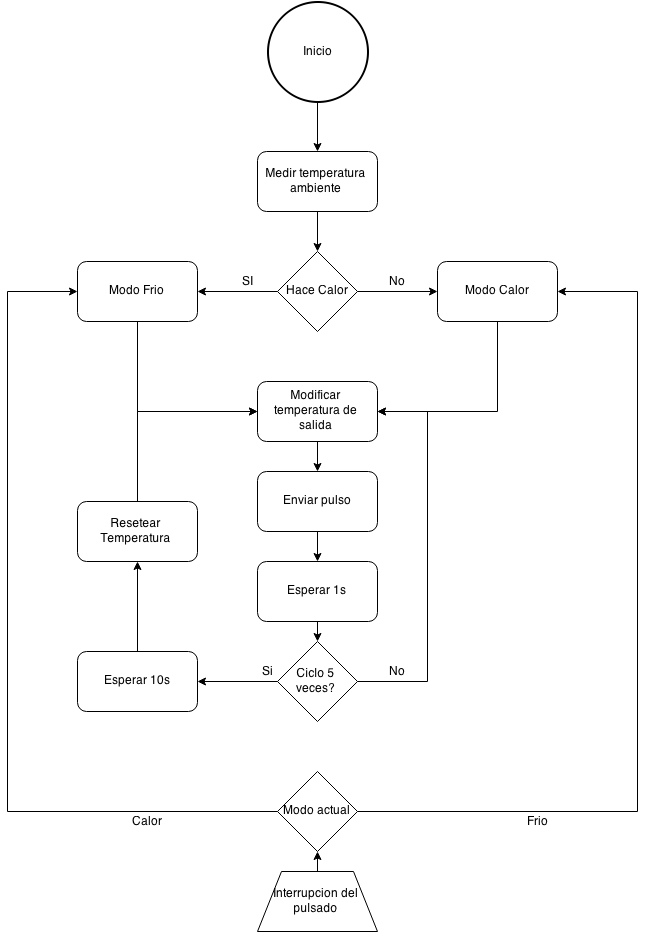
\includegraphics[scale=0.65]{./imagenes/diagrama_de_flujo.png}
\caption{Diagrama de flujo del proceso}
 \label{fig:diag_flujo}
\end{center}
\end{figure}

\subsection{Diagrama de Bloques}

\ifx\du\undefined
  \newlength{\du}
\fi
\setlength{\du}{15\unitlength}
\begin{tikzpicture}
\pgftransformxscale{1.000000}
\pgftransformyscale{-1.000000}
\definecolor{dialinecolor}{rgb}{0.000000, 0.000000, 0.000000}
\pgfsetstrokecolor{dialinecolor}
\definecolor{dialinecolor}{rgb}{1.000000, 1.000000, 1.000000}
\pgfsetfillcolor{dialinecolor}
\pgfsetlinewidth{0.100000\du}
\pgfsetdash{}{0pt}
\pgfsetdash{}{0pt}
\pgfsetbuttcap
\pgfsetmiterjoin
\pgfsetlinewidth{0.100000\du}
\pgfsetbuttcap
\pgfsetmiterjoin
\pgfsetdash{}{0pt}
\definecolor{dialinecolor}{rgb}{1.000000, 1.000000, 1.000000}
\pgfsetfillcolor{dialinecolor}
\fill (5.634315\du,11.087500\du)--(10.434315\du,11.087500\du)--(12.034315\du,11.087500\du)--(12.034315\du,10.100000\du)--(15.234315\du,12.075000\du)--(12.034315\du,14.050000\du)--(12.034315\du,13.062500\du)--(5.634315\du,13.062500\du)--cycle;
\definecolor{dialinecolor}{rgb}{0.000000, 0.000000, 0.000000}
\pgfsetstrokecolor{dialinecolor}
\draw (5.634315\du,11.087500\du)--(10.434315\du,11.087500\du)--(12.034315\du,11.087500\du)--(12.034315\du,10.100000\du)--(15.234315\du,12.075000\du)--(12.034315\du,14.050000\du)--(12.034315\du,13.062500\du)--(5.634315\du,13.062500\du)--cycle;
\pgfsetbuttcap
\pgfsetmiterjoin
\pgfsetdash{}{0pt}
\definecolor{dialinecolor}{rgb}{0.000000, 0.000000, 0.000000}
\pgfsetstrokecolor{dialinecolor}
\draw (5.634315\du,11.087500\du)--(10.434315\du,11.087500\du)--(12.034315\du,11.087500\du)--(12.034315\du,10.100000\du)--(15.234315\du,12.075000\du)--(12.034315\du,14.050000\du)--(12.034315\du,13.062500\du)--(5.634315\du,13.062500\du)--cycle;
\definecolor{dialinecolor}{rgb}{1.000000, 1.000000, 1.000000}
\pgfsetfillcolor{dialinecolor}
\pgfpathellipse{\pgfpoint{18.196332\du}{12.131160\du}}{\pgfpoint{2.928364\du}{0\du}}{\pgfpoint{0\du}{2.251682\du}}
\pgfusepath{fill}
\pgfsetlinewidth{0.100000\du}
\pgfsetdash{}{0pt}
\pgfsetdash{}{0pt}
\pgfsetmiterjoin
\definecolor{dialinecolor}{rgb}{0.000000, 0.000000, 0.000000}
\pgfsetstrokecolor{dialinecolor}
\pgfpathellipse{\pgfpoint{18.196332\du}{12.131160\du}}{\pgfpoint{2.928364\du}{0\du}}{\pgfpoint{0\du}{2.251682\du}}
\pgfusepath{stroke}
% setfont left to latex
\definecolor{dialinecolor}{rgb}{0.000000, 0.000000, 0.000000}
\pgfsetstrokecolor{dialinecolor}
\node at (18.196332\du,12.326160\du){};
\definecolor{dialinecolor}{rgb}{1.000000, 1.000000, 1.000000}
\pgfsetfillcolor{dialinecolor}
\fill (26.779722\du,13.760051\du)--(26.779722\du,20.160051\du)--(34.579722\du,20.160051\du)--(34.579722\du,13.760051\du)--cycle;
\pgfsetlinewidth{0.100000\du}
\pgfsetdash{}{0pt}
\pgfsetdash{}{0pt}
\pgfsetmiterjoin
\definecolor{dialinecolor}{rgb}{0.000000, 0.000000, 0.000000}
\pgfsetstrokecolor{dialinecolor}
\draw (26.779722\du,13.760051\du)--(26.779722\du,20.160051\du)--(34.579722\du,20.160051\du)--(34.579722\du,13.760051\du)--cycle;
% setfont left to latex
\definecolor{dialinecolor}{rgb}{0.000000, 0.000000, 0.000000}
\pgfsetstrokecolor{dialinecolor}
\node at (30.679722\du,17.155051\du){};
\definecolor{dialinecolor}{rgb}{1.000000, 1.000000, 1.000000}
\pgfsetfillcolor{dialinecolor}
\fill (26.873656\du,28.957539\du)--(26.873656\du,36.107539\du)--(34.473656\du,36.107539\du)--(34.473656\du,28.957539\du)--cycle;
\pgfsetlinewidth{0.100000\du}
\pgfsetdash{}{0pt}
\pgfsetdash{}{0pt}
\pgfsetmiterjoin
\definecolor{dialinecolor}{rgb}{0.000000, 0.000000, 0.000000}
\pgfsetstrokecolor{dialinecolor}
\draw (26.873656\du,28.957539\du)--(26.873656\du,36.107539\du)--(34.473656\du,36.107539\du)--(34.473656\du,28.957539\du)--cycle;
% setfont left to latex
\definecolor{dialinecolor}{rgb}{0.000000, 0.000000, 0.000000}
\pgfsetstrokecolor{dialinecolor}
\node at (30.673656\du,32.727539\du){};
\definecolor{dialinecolor}{rgb}{1.000000, 1.000000, 1.000000}
\pgfsetfillcolor{dialinecolor}
\fill (10.342894\du,30.273590\du)--(10.342894\du,34.872616\du)--(15.319413\du,34.872616\du)--(15.319413\du,30.273590\du)--cycle;
\pgfsetlinewidth{0.100000\du}
\pgfsetdash{}{0pt}
\pgfsetdash{}{0pt}
\pgfsetmiterjoin
\definecolor{dialinecolor}{rgb}{0.000000, 0.000000, 0.000000}
\pgfsetstrokecolor{dialinecolor}
\draw (10.342894\du,30.273590\du)--(10.342894\du,34.872616\du)--(15.319413\du,34.872616\du)--(15.319413\du,30.273590\du)--cycle;
% setfont left to latex
\definecolor{dialinecolor}{rgb}{0.000000, 0.000000, 0.000000}
\pgfsetstrokecolor{dialinecolor}
\node at (12.831153\du,32.768103\du){};
% setfont left to latex
\definecolor{dialinecolor}{rgb}{0.000000, 0.000000, 0.000000}
\pgfsetstrokecolor{dialinecolor}
\node[anchor=west] at (6.722382\du,12.332936\du){Temperatura ambiente};
% setfont left to latex
\definecolor{dialinecolor}{rgb}{0.000000, 0.000000, 0.000000}
\pgfsetstrokecolor{dialinecolor}
\node[anchor=west] at (16.423109\du,12.316516\du){Termometro};
% setfont left to latex
\definecolor{dialinecolor}{rgb}{0.000000, 0.000000, 0.000000}
\pgfsetstrokecolor{dialinecolor}
\node[anchor=west] at (28.159011\du,17.266117\du){Microcontrolador};
% setfont left to latex
\definecolor{dialinecolor}{rgb}{0.000000, 0.000000, 0.000000}
\pgfsetstrokecolor{dialinecolor}
\node[anchor=west] at (28.414037\du,32.231066\du){Circuito regulador};
% setfont left to latex
\definecolor{dialinecolor}{rgb}{0.000000, 0.000000, 0.000000}
\pgfsetstrokecolor{dialinecolor}
\node[anchor=west] at (28.414037\du,33.031066\du){de corriente};
% setfont left to latex
\definecolor{dialinecolor}{rgb}{0.000000, 0.000000, 0.000000}
\pgfsetstrokecolor{dialinecolor}
\node[anchor=west] at (11.805850\du,32.785235\du){Peltier};
\pgfsetlinewidth{0.100000\du}
\pgfsetdash{}{0pt}
\pgfsetdash{}{0pt}
\pgfsetbuttcap
\pgfsetmiterjoin
\pgfsetlinewidth{0.100000\du}
\pgfsetbuttcap
\pgfsetmiterjoin
\pgfsetdash{}{0pt}
\definecolor{dialinecolor}{rgb}{1.000000, 1.000000, 1.000000}
\pgfsetfillcolor{dialinecolor}
\fill (5.613908\du,20.979783\du)--(10.413908\du,20.979783\du)--(12.013908\du,20.979783\du)--(12.013908\du,19.992283\du)--(15.213908\du,21.967283\du)--(12.013908\du,23.942283\du)--(12.013908\du,22.954783\du)--(5.613908\du,22.954783\du)--cycle;
\definecolor{dialinecolor}{rgb}{0.000000, 0.000000, 0.000000}
\pgfsetstrokecolor{dialinecolor}
\draw (5.613908\du,20.979783\du)--(10.413908\du,20.979783\du)--(12.013908\du,20.979783\du)--(12.013908\du,19.992283\du)--(15.213908\du,21.967283\du)--(12.013908\du,23.942283\du)--(12.013908\du,22.954783\du)--(5.613908\du,22.954783\du)--cycle;
\pgfsetbuttcap
\pgfsetmiterjoin
\pgfsetdash{}{0pt}
\definecolor{dialinecolor}{rgb}{0.000000, 0.000000, 0.000000}
\pgfsetstrokecolor{dialinecolor}
\draw (5.613908\du,20.979783\du)--(10.413908\du,20.979783\du)--(12.013908\du,20.979783\du)--(12.013908\du,19.992283\du)--(15.213908\du,21.967283\du)--(12.013908\du,23.942283\du)--(12.013908\du,22.954783\du)--(5.613908\du,22.954783\du)--cycle;
% setfont left to latex
\definecolor{dialinecolor}{rgb}{0.000000, 0.000000, 0.000000}
\pgfsetstrokecolor{dialinecolor}
\node[anchor=west] at (6.675041\du,22.238360\du){Temperatura corporal};
\definecolor{dialinecolor}{rgb}{1.000000, 1.000000, 1.000000}
\pgfsetfillcolor{dialinecolor}
\pgfpathellipse{\pgfpoint{18.244744\du}{22.071211\du}}{\pgfpoint{2.928364\du}{0\du}}{\pgfpoint{0\du}{2.251682\du}}
\pgfusepath{fill}
\pgfsetlinewidth{0.100000\du}
\pgfsetdash{}{0pt}
\pgfsetdash{}{0pt}
\pgfsetmiterjoin
\definecolor{dialinecolor}{rgb}{0.000000, 0.000000, 0.000000}
\pgfsetstrokecolor{dialinecolor}
\pgfpathellipse{\pgfpoint{18.244744\du}{22.071211\du}}{\pgfpoint{2.928364\du}{0\du}}{\pgfpoint{0\du}{2.251682\du}}
\pgfusepath{stroke}
% setfont left to latex
\definecolor{dialinecolor}{rgb}{0.000000, 0.000000, 0.000000}
\pgfsetstrokecolor{dialinecolor}
\node at (18.244744\du,22.266211\du){};
% setfont left to latex
\definecolor{dialinecolor}{rgb}{0.000000, 0.000000, 0.000000}
\pgfsetstrokecolor{dialinecolor}
\node[anchor=west] at (16.539171\du,22.238360\du){Termocupla};
\pgfsetlinewidth{0.100000\du}
\pgfsetdash{}{0pt}
\pgfsetdash{}{0pt}
\pgfsetbuttcap
{
\definecolor{dialinecolor}{rgb}{0.000000, 0.000000, 0.000000}
\pgfsetfillcolor{dialinecolor}
% was here!!!
\definecolor{dialinecolor}{rgb}{0.000000, 0.000000, 0.000000}
\pgfsetstrokecolor{dialinecolor}
\draw (20.603338\du,13.485307\du)--(26.779722\du,16.960051\du);
}
\pgfsetlinewidth{0.100000\du}
\pgfsetdash{}{0pt}
\pgfsetdash{}{0pt}
\pgfsetbuttcap
{
\definecolor{dialinecolor}{rgb}{0.000000, 0.000000, 0.000000}
\pgfsetfillcolor{dialinecolor}
% was here!!!
\definecolor{dialinecolor}{rgb}{0.000000, 0.000000, 0.000000}
\pgfsetstrokecolor{dialinecolor}
\draw (21.173108\du,22.071211\du)--(26.779722\du,16.960051\du);
}
\pgfsetlinewidth{0.100000\du}
\pgfsetdash{}{0pt}
\pgfsetdash{}{0pt}
\pgfsetbuttcap
{
\definecolor{dialinecolor}{rgb}{0.000000, 0.000000, 0.000000}
\pgfsetfillcolor{dialinecolor}
% was here!!!
\definecolor{dialinecolor}{rgb}{0.000000, 0.000000, 0.000000}
\pgfsetstrokecolor{dialinecolor}
\draw (30.679722\du,20.160051\du)--(30.673656\du,28.957539\du);
}
\pgfsetlinewidth{0.100000\du}
\pgfsetdash{}{0pt}
\pgfsetdash{}{0pt}
\pgfsetbuttcap
{
\definecolor{dialinecolor}{rgb}{0.000000, 0.000000, 0.000000}
\pgfsetfillcolor{dialinecolor}
% was here!!!
\definecolor{dialinecolor}{rgb}{0.000000, 0.000000, 0.000000}
\pgfsetstrokecolor{dialinecolor}
\draw (26.831594\du,32.541273\du)--(15.369114\du,32.567333\du);
}
\end{tikzpicture}


\begin{thebibliography}{9}

\bibitem{embrlabs}
  \ULurl{http://www.embrlabs.com/}

\bibitem{Make It Wearable}
  \ULurl{https://youtu.be/sDZHITVfYrI}
  
\bibitem{video MIT}
  \ULurl{https://youtu.be/kvUMCip-r4A}

\end{thebibliography}

\end{document}
